\documentclass{school-22.211-notes}
\date{April 25, 2012}

\begin{document}
\maketitle

\lecture{Point Kinetics Without Feedback}
\topic{Physics of Delayed Neutrons}
\textbf{Prompt neutrons}: more than 99\% of all neutrons are emitted in $<10^{-10}$s after the fission (prompt neutron lifetime in a PWR is about $2 \times 10^{-5}$ sec). Example: A reactor was operated at 1W, a control rod was moved to produce an excess reactivity of $0.0005 \Delta k$, what would the power be 1s later? 
\begin{align}
P(t) &= P_0 (1.0005)^{t/(2\times 10^{-5})} = 1 W (1.0005)^{1/(2\times 10^{-5})} = 70,000 MW 
\end{align}
The above calculation means that this reactor would be virtually impossible to control! Fortunately, delayed netrons exist and the reactor time constant depend on more than just prompt neutron lifetime. 

\textbf{Delayed neutrons}:
\begin{enumerate}
\item Measurement: delayed neutrons can be measured by counting neutrons emission after a pulsed irradiation of a pure U235 foil. Burst measurement represents the amount of prompt neutrons; saturated measurement represents the total amount of neutrons. 
\item Emission: delayed neutrons are emitted through the decay of fission products, of which Br-37 is a dominant FP that emits delayed neutrons. 
\item Delayed yields depend on fissioning species and neutron energy (keep in mind that U238 produce 4\% delayed neutron per fission, more than U235's 1.7\% delayed neutron per fission, making U238 a very important isotope when it comes to delayed neutrons). 
  \begin{itemize}
  \item Absolute yield: number of delayed neutrons per fission; unit: 1/fission. 
  \item Relative yield: absolute yield of an isotope divided by total absolute yield by all isotopes; 
  \item Delayed neutron fraction: absolute yield divided by $\bar{\nu}$. Number of delayed neutrons devided by number of total fission neutrons. 
  \end{itemize}
  \begin{table}[ht]
    \centering
    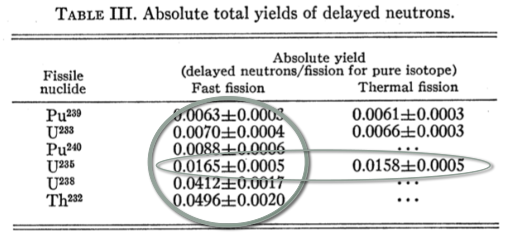
\includegraphics[width=4in]{images/pke/abs-yield.png}
    \caption{Absolute Total Yields of Delayed Neutrons} \label{abs-yield} 
  \end{table}
\item Modern trend: makes the 6-group to 8-group, and each group has a fixed decay constants (the one that dominants in the group, that is, largest half-life). This way, all isotopes have the same half-life for the same group; but different isotopes would still have different delayed neutron fraction. Remember the terms circled in blue.  
\item Delayed neutrons spectrum vs. energy: average prompt neutron emission energy is 2 MeV; average delayed neutron emission energy is 0.4 MeV. Both spectrum comes out to be Maxwellian, except the delayed one is shifted as in Fig.~\ref{fission-spec}. Delayed neutron comes out in the thermal energy range, which makes them more likely to fission. 
  \begin{figure}[ht]
    \centering
    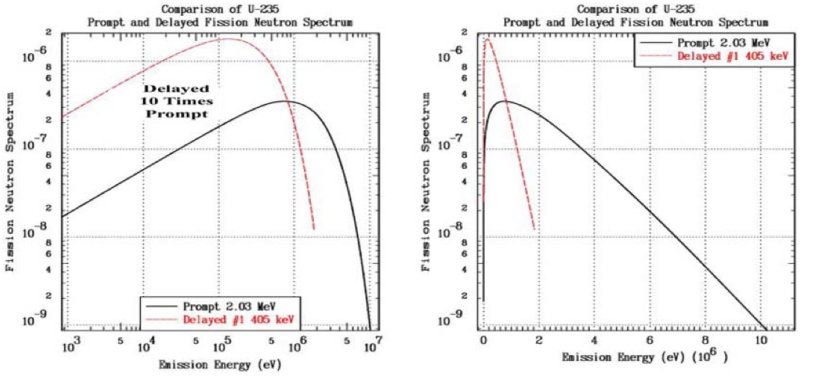
\includegraphics[width=4in]{images/pke/fission-spec.png}
    \caption{Prompt and Delayed Fission Neutron Spectrum} \label{fission-spec} 
  \end{figure}
\item Delayed energy group: neutron spectra have similar shapes for all delayed groups. However different energy groups have different mean energies. 
  \begin{figure}[ht]
    \centering
    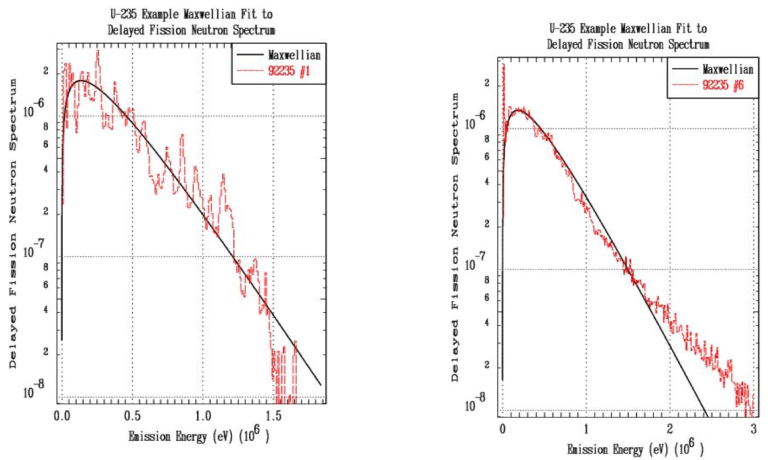
\includegraphics[width=4in]{images/pke/delayed-fission-spec.png}
    \caption{Delayed Fission Neutron Spectrum} \label{delayed-fission-spec} 
  \end{figure}
\item Take-away message: delayed neutron spectra vary only slightly for different fissioning nuclides; but the spectra depends significantly on the delayed neutron group. 
\end{enumerate}

\clearpage
\topic{Derivation of Point Kinetics Equations (PKE)}
In steady-state transport or diffusion equation, we do not treat delayed neutrons directly. But the fission emission spectrum must be properly weighted with prompt and delayed contributions. Notice one issue is, we need fission rates to get $\chi$, and we need $\chi$ to get fission rates, so the real way to solve the balance equation is to iterate, though this is not how it is done normally.
\begin{enumerate}
\item We start from the diffusion equation: \hi{The steady-state diffusion equation}\footnote{Know this for the final}: 
\small
\begin{align}
& - \divergence D(\vecr, E, t) \gradient \phi(\vecr, E, t) + \Sigma_t (\vecr, E, t) \phi(\vecr, E, t) = \int_0^{\infty} \Sigma_s (\vecr, E'\to E, t) \phi(\vecr, E', t) \dE' \\
&+ \Sum_j \chi_T^j (E) \int_0^{\infty} \nu \Sigma_p^j (\vecr, E', t) \phi(\vecr, E', t) \dE' + Q(\vecr, E, t) 
\end{align}
\normalsize

\item \hi{The time-dependent neutron diffusion equation}: where $\beta^j = \Sum_i \beta_i^j$ is the delayed fission fraction (0.66\% for instance), 
  \begin{align}
    \ppt \left[ \frac{1}{v} \phi(\vecr, E, t) \right] &= \divergence D(\vecr, E, t) \gradient \phi(\vecr, E, t) - \Sigma_t (\vecr, E, t) \phi(\vecr, E, t) \\
    & + \int_0^{\infty} \Sigma_s (\vecr, E'\to E, t) \phi(\vecr, E', t) \dE' \\
    &+ \Sum_j \chi_p^j (E) (1-\beta^j) \int_0^{\infty} \nu \Sigma_f^j (\vecr, E', t) \phi(\vecr, E', t) \dE' \\
    &+ \Sum_i \chi_d^i (E) \lambda_i C_i (\vecr, t) + Q(\vecr, E, t)\\
    \ppt C_i (\vecr, t) &= \Sum_j \beta_i^j \int_0^{\infty} \nu \Sigma_p^j (\vecr, E', t) \phi(\vecr, E', t) \dE' - \lambda_i C_i (\vecr, t) 
  \end{align}

\item Assume that flux can be separated into a space/energy term and a time-dependent term: $\phi(\vecr, E, t) = S(\vecr, E) T(t)$. Plug it into the above expressions. 
\begin{figure}[ht]
  \centering
  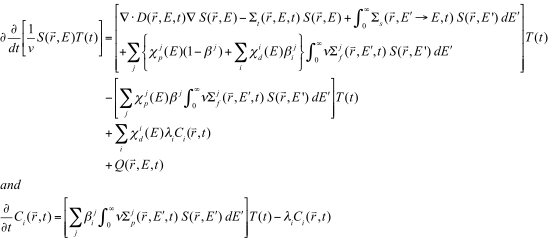
\includegraphics[width=5in]{images/pke/pke1.png}
\end{figure}

\clearpage
\item Integrate over all space and energy and normalize to $\int \dE \int \dr \frac{1}{v} S(\vecr, E) = 1.0$, 
\begin{figure}[ht]
  \centering
  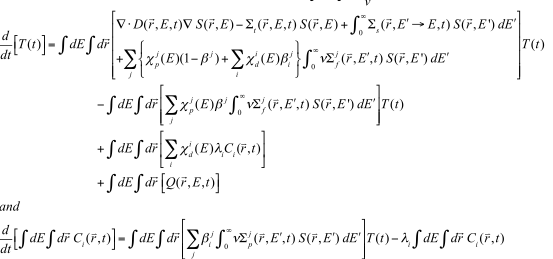
\includegraphics[width=4.5in]{images/pke/pke2.png}
\end{figure}

\item If we define the following terms, 
\begin{figure}[ht]
  \centering
  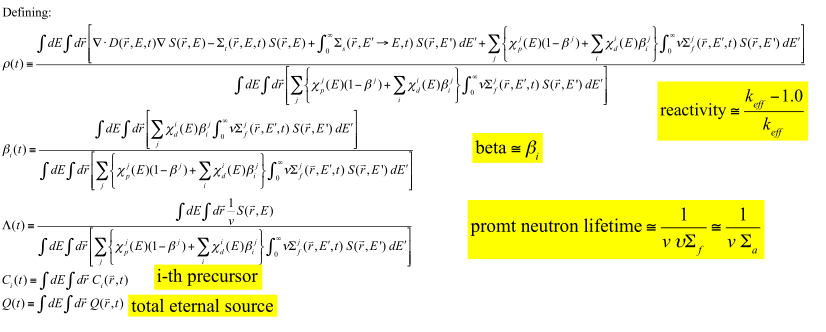
\includegraphics[width=6in]{images/pke/pke3.png}
\end{figure}
where the top of $\rho(t)$ is the diffusion equation, which is zero for steady state.  The bottom of rho: fission rate (if all the neutrons show up instatenously, the bottom would be the fission rate). The prompt neutron life $\Gamma \sim 1/v$ of shape divided by almost-instantenous-fission-rate. 

\item Then we get the point kinetics equations,
\begin{align}
\Aboxed{ \ddt T(t) &= \frac{\rho(t) - \Sum_i \beta_i (t) }{\Gamma (t)} T(t) + \Sum_i \lambda_i C_i (t) + Q(t) } \\
\Aboxed{ \ddt C_i (t) &= \frac{\beta_i (t)}{\Lambda (t)} T(t) - \lambda_i C_i (t) } 
\end{align}

\item For a steady state solution, at power level $T_0$, we know, 
  \eqn{\ddt C_i (0) = 0 \Rightarrow C_i (0) = \frac{\beta_i}{\Gamma \lambda_i} T_0 }
  \eqn{\ddt T(0) = 0 \Rightarrow \rho(0) = 0 }
Under the assumption that there is no feedback (e.g., the reactor is operating at low enough flux, no feedback, coefficients are independent of solution), if $\rho(t)$ is known, one can solve for reactor power as a function of time.

\item The matrix form of the equation system, 
\begin{figure}[ht]
  \centering
  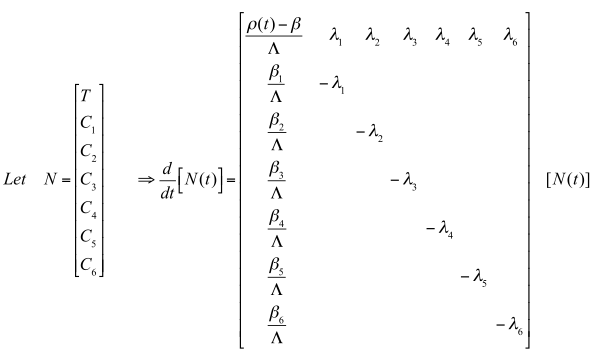
\includegraphics[width=4in]{images/pke/matrix-form.png}
\end{figure}
\end{enumerate}

\clearpage
\topic{Simple Matlab Methods for Solving PKEs}

\begin{enumerate}
\item Instantaneous reactor scram ($\rho = - 8 \beta$): 

Question: does the 8 group happen to have half-lives from large to small? 
\item Two seconds rod drop ($\rho = - 8 \beta$):

\item Instantaneous rod withdraw ($\rho = 0.1 \beta$): 
The reactor wants to response immediately (hence it jumps) but it does not have enough delayed neutron to sustain that increase, hence the jump is not enough and it will increase for the rest of the way. To estimate the prompt jump, we do the prompt jump approximation (easy to do in 1 group)

\item 4b: if we wait long enough, we reach secular equilibrium between power and precursor rate that the precursor rates have the same shapes as the power, altough the rates may be off by a factor. 

\item 

\item Power does not come back to the same level, because we are solving for an eigenvalue problem, and what the asymptotic power is depends on how to get there. In the withdrawal case, the precursor builds up and is continuing to build up during the second phase, so the power ends up higher than initially. 


\item Super-prompt criticality: when reactivity exceeds beta, reactivity does not have to wait for the delayed neutrons anymore, changes can happen instantaneously.  
\end{enumerate}



\clearpage
\topic{Understanding Reactor Behavior with PKEs}
\subtopic{Negative Reactivity Excursions}


\subtopic{Positive Reactivity Excursions}


\subtopic{Prompt Excursions}

\clearpage
\topic{Approximate Solutions}
\subtopic{Prompt-Jump Approximations}


\subtopic{In-hour Equations: THe Simpliest Inverse Kinetics Application}
From the PKEs, know how to derive the In-hour Equation: 
\begin{align}
\Aboxed{ \rho &= \omega \Lambda + \Sum_i \frac{\beta_i \omega}{\omega + \lambda_i}}
\end{align}
That is, knowing every other term, we can back out reactivity $\rho$ assuming there is no feedback. The steps are: 


\clearpage
\topic{Reactivity Units}
\begin{table}[ht]
  \centering
  \begin{tabular}{|c|c|c|}
    $\Delta k$ & actual units of PKEs & 0.01 \\
    \% $\Delta k$ & & 1/% \\
  \end{tabular}
\end{table}

\clearpage
\topic{Derivation of Inverse Kinetics Equations (IK)}
Assume we know the amplitude function $T(t)$, we can solve for the pre-cursor function $C(t)$; then plugging back in the PKEs, we can get $\rho(t)$. 



\clearpage
\topic{Experimental Applications of IK}
\subtopic{PWR Boration/Dilution}

The red curve is measured by detectors. Prompt neutron life time is so short, so that even spatial distribution flux changes a lot, we can assume that it stabalizes already at each rod drop. 

Disadvantages: time concern; boration dilution increases cost with waste disposal.  

Alternatives: we use General Inverse Kinetics to get around about it. 

\subtopic{SCRAM/Rod Drop Analysis}
From scram, we measure power change, infer $T(t)$, and estimate reactivity.

The rough method use Prompt Jumpt Approximation,


More accurately, we need to model all the neutron sources, including ($\alpha,n$) reactions etc. It comes out to be, 


In reality, there are noisy signals in measured power and reactivity data; we need to smooth them out with a fitted function before we can apply IK with external neutron sources. 

This technique is not used in the US that much because it is harsh your system and it requires work to bring the system back to critical. But it is one of the best ways to demonstrate to the licensing committee that a reactor is capable to scram.  

\subtopic{Dynamic Rod Worth}
We start with a critical reactor, and drive a control rod in and out and repeat with a different rod. The advantages are: no need to do boron dilution, and it takes 15 mins for each rod. This technique is widely used by Westinghouse to estimate their rod worth. 




Alternatively, we can do sub-critical source multiplication, that is, IK with a source in the reactor. This way we don't even need to start with a critical reactor. This technique has only been used in experimental reactors but not so much in power reactors because it requires detailed knowledge about the source distribution. 

\subtopic{Oscillator Sample Worth Measurements}


\clearpage
\topic{Summary}
Shape function $S(\vecr, E)$, amplitude function, $T(t)$. 

PKT: the top of $\rho$ is just the steady-state diffusion equation; at steady state, $\keff = 1, \rho = 0$. 

There are four fundamental thing: diffusion equation, point-kinetics equation, derive the prompt-jump approximation, derive the in-hour equation. 


Questions:  p.12, steps. 
p.19, why don't image 1 match image 4: because step sizes are not uniform. 
p.27, 
p.29

\end{document}
